\section{Feature-First Block Model}

We propose a novel generative model for labelled networks -- which we call the feature-first block model (FFBM),
illustrated in Figure~\ref{fig:ffbm}.
Let $N$ denote the number of vertices, $B$ the number of blocks
and $D$ the number of features associated with each vertex.
We write $X$ for the $N\times D$ {\em feature matrix} containing
the feature vectors $\{x_i\}_{i=1}^{N}$ 
as its rows.
%
For the FFBM, we start with the feature matrix $X$ and generate a random
vector of block memberships $b \in [B]^N$ -- noting the notation $[K] = \{1, 2 \dots K\}$. For each vertex $i$, the
block membership $b_i\in[B]$ is generated based on the feature
vector $x_i$, independently between vertices, 
$p(b| X, \theta) = \prod_{i \in [N]} \phi_{b_i} (x_i; \theta)$.
%
\begin{figure}[!ht]
	\centering
%   IWSM Template does not support TIKZ
%	\begin{tikzpicture}[
%		roundnode/.style={circle, draw=black, minimum size=7mm},
%		squarednode/.style={rectangle, draw=black, minimum size=7mm}
%		]
%		% nodes
%		\node[roundnode] (X) at (0, 0) {$X$};
%		\node[squarednode] (b) at (3, 0) {$b$};
%		\node[roundnode] (A) at (6, 0) {$A$};
%		
%		% arrows
%		\draw[->] (X.east) -- node[above] {$\theta$} (b.west);
%		\draw[->] (b.east) -- node[above] {$\psi$}(A.west);
%	\end{tikzpicture}
	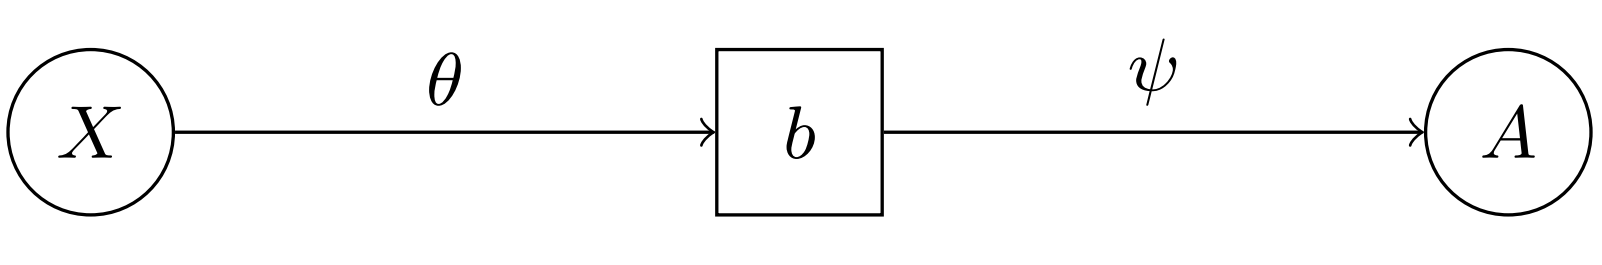
\includegraphics[width=0.8\textwidth]{img/ffbm.png}
	\caption{The Feature-First Block Model (FFBM)}
	\label{fig:ffbm}
\end{figure}

Once the block memberships $b$ have been generated, we then draw the 
adjacency matrix of the graph, $A$, from the microcanonical DC-SBM, Peixoto (2017), with additional parameters 
$\psi$,
$
	A \sim \textrm{DC-SBM}_{\textrm{MC}} (b, \psi).
	\label{eqn:A-generation}
$
Priors on the parameters $\theta$ and $\psi$ are chosen to complete the Bayesian framework.
